%%%%%%%
% Ch3       %
%%%%%%%

\chapter{Thyristor converters}
	In this chapter we will focus on rectifiers/inverters with thyristors and a controllable and invertible output. They are bridges obtained by replacing the diodes of the bridges studied in Chapter 2 by thyristors. We will also study \textbf{half-controlled bridges}. These half-controlled bridges are composed of diodes and thyristors. Consequently they are controllable but irreversible. Finally we will study AC choppers and cycloconverters, that will allow us to do AC/AC conversions without going through the DC. Choppers are composed of \textbf{triacs}, \textbf{bidirectional and semi-controllable switches}. 
	
	\section{Characteristics of thyristors}
		\begin{wrapfigure}[8]{l}{7cm}
		\vspace{-5mm}
		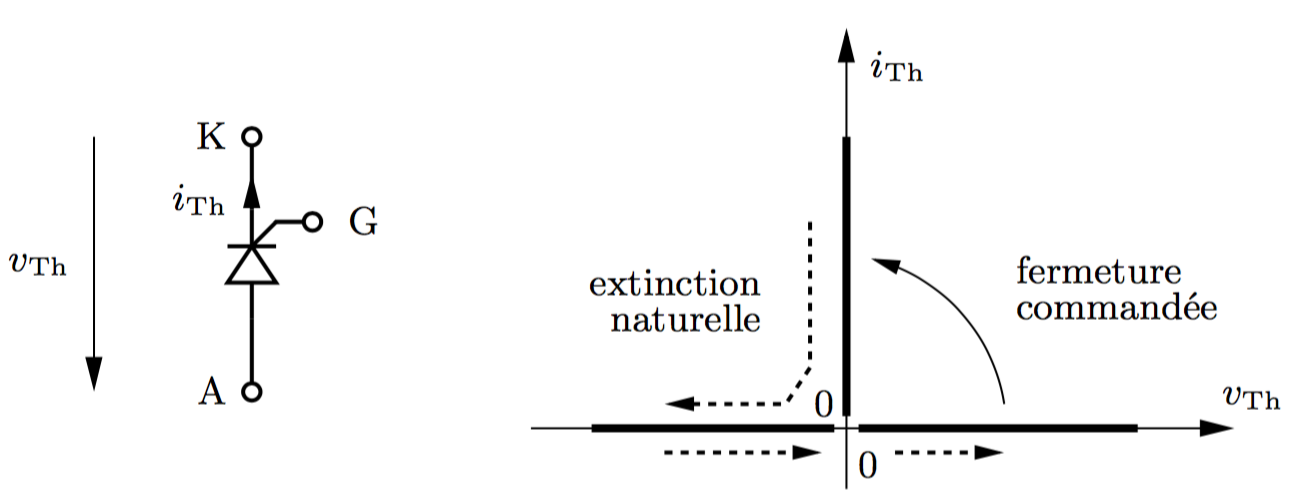
\includegraphics[scale=0.3]{ch3/1}
		\captionof{figure}{} 
		\label{fig:3.1}
		\end{wrapfigure}
		A thyristor (also called SCR: Silicon Controlled Rectifier) is represented in \autoref{fig:3.1}. During conduction the current $i_{Th} > 0$ flows from the anode A to the cathode K and the \textbf{gate G} allows us to choose the starting moment. It has the same behaviour as a diode. When it is \textbf{inversely biased} ($V_{AK}<0$), there is a leakage current $<0$ that can be neglected most of the times. When it is \textbf{directly biased}, it will only conduct when positive current impulsions go into the gate. As the diode does, the thyristor turns itself off when there is no current $i_{AK}$ going through it. That is why they are called \textbf{semi-controllable}. We can make them fully-controllable by adding an extra commutation circuit, which will increase the complexity of the device and will increase the losses. \\
		
		The direct and inverse voltage and the conduction current a thyristor can endure can go up to some \textbf{kilo} volts/amperes. The voltage drop due to conduction is of more or less 1 V and it is referred to using $V_{Th,on}$ and $R_{Th,on}$. The frequency capability is nevertheless very limited. In the case of the grid that is not a problem but it will be problematic when frequencies becomes greater than some hundreds of Hertz. 


	\section{Elementary circuits with one or two thyristors}
		\subsection{Circuit with one thyristor and a resistance}
		    When we have an ideal AC voltage source, the current $i_{ac}(t) = i_{dc}(t)$. During positive alternations, the thyristor is in direct-bias. The impulsions in the gate are given with a delay $\alpha$ [rad] called \textbf{firing angle} that ranges from 0 to $\pi$. When $v_{ac}$ becomes negative, $i_{dc}$ and $v_{dc}$ will become negative too and the thyristor will turn itself off (inverse-bias). That circumstance is represented in \autoref{fig:3.2}. The average value of the rectified voltage will be:
			\begin{equation}
				V_{dc} = \frac{1}{2\pi}\int _\alpha ^\pi \sqrt{2} V_{ac} \sin \omega t \, d\omega t = \frac{\sqrt{2}}{\pi} \frac{1+\cos \alpha}{2} V_{ac}.
			\end{equation}
			
			\begin{minipage}{0.49\textwidth}
				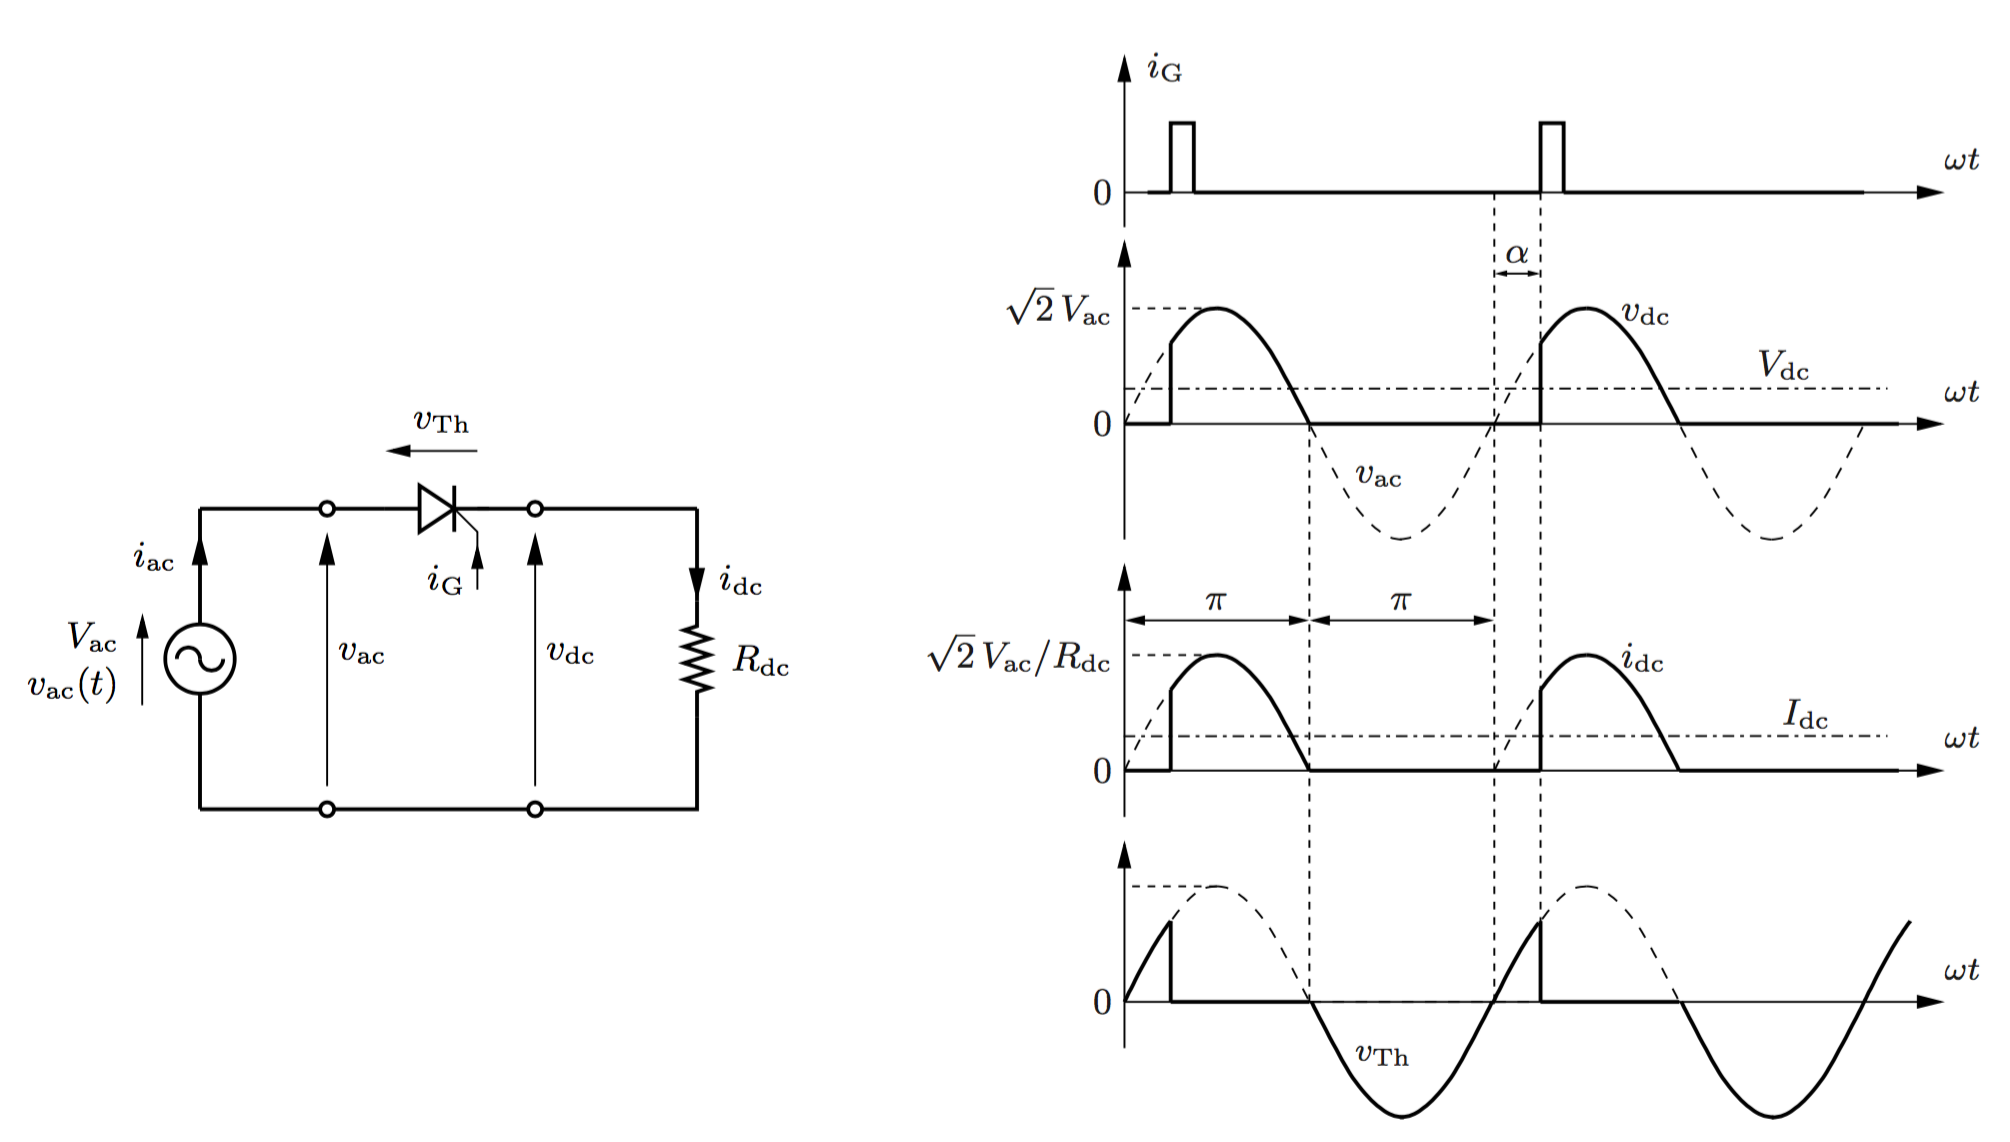
\includegraphics[scale=0.2]{ch3/2}
				\captionof{figure}{}
				\label{fig:3.2}
			\end{minipage}
			\begin{minipage}{0.49\textwidth}
				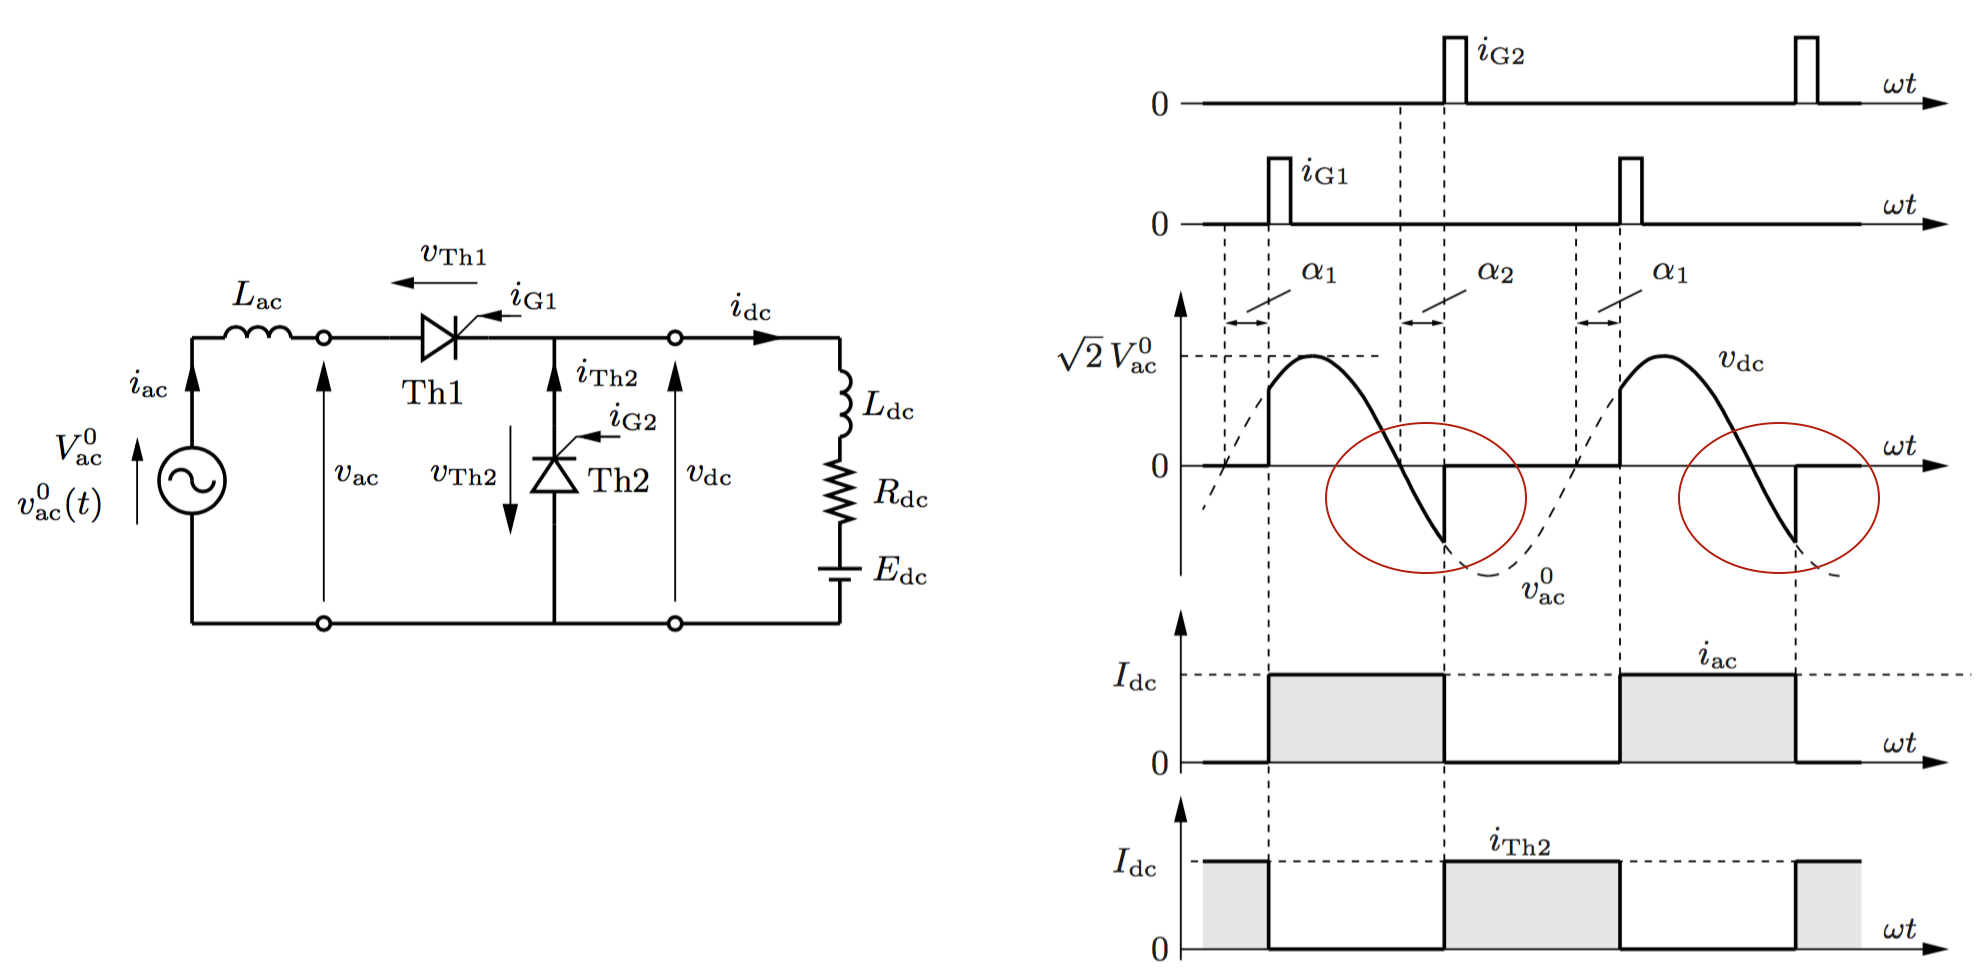
\includegraphics[scale=0.21]{ch3/3}
				\captionof{figure}{}
				\label{fig:3.3}
			\end{minipage}
			
		\subsection{Circuit with a rectifier thyristor and a free-wheeling thyristor}
		This distribution is shown in \autoref{fig:3.3}, where we can see 2 diodes Th1 and Th2. We will distinguish two different cases depending on the source.  
			
			\subsubsection{With ideal voltage source (without inductance)}
				The wave shapes when $L_{ac} = 0, L_{dc} = \infty$ are drawn in \autoref{fig:3.3}. We can see that the conduction interval of Th1 depends on 2 angles $\alpha _1$ and $\alpha _2$. When $i_{dc}$ flows in Th2, $v_{dc} = 0$. We consider that commutation is instantaneous. We remark that $v_{dc}$ becomes negative until the current impulsion $i_{G2}$. As a matter of fact, the 2 thyristors cannot conduct at the same time, otherwise $v_{ac} = v_{Th1} - v_{Th2}$. We can see that if $v_{ac} < 0$ and Th1 conducts, then $v_{ac} = -v_{Th2} = v_{dc}$. The average output voltage is: 
				\begin{equation}
					V_{dc} = \frac{1}{2\pi} \int _{\alpha _1} ^{\pi + \alpha _2} \sqrt{2} V_{ac}^0\sin \omega t \, d\omega t = \frac{\sqrt{2}}{\pi} \frac{\cos \alpha _1 + \cos \alpha _2}{2} V_{ac}^0.
 				\end{equation}
		
			\subsubsection{With non-ideal voltage source (with inductance)}
				\begin{wrapfigure}[12]{l}{6cm}
				\vspace{-5mm}
				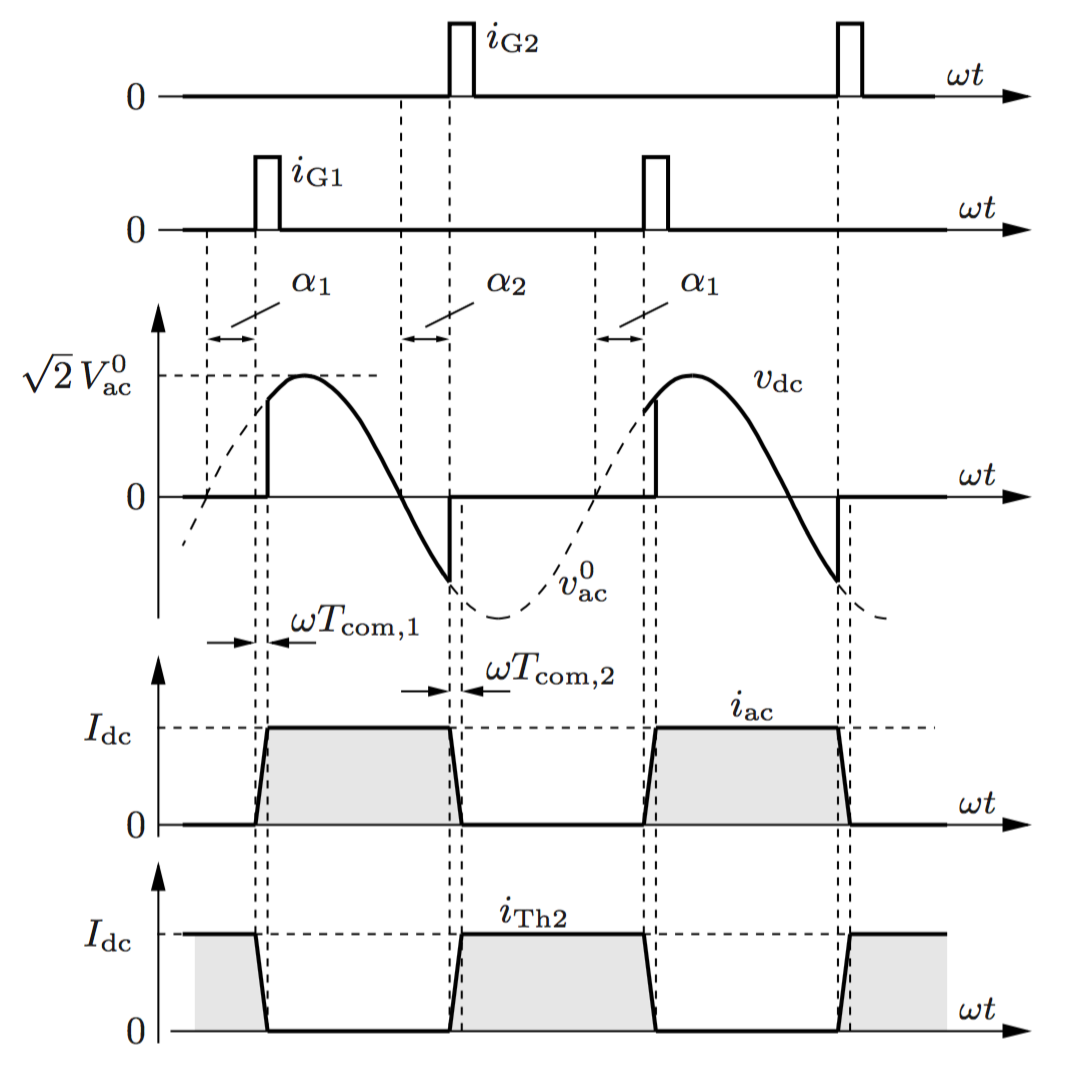
\includegraphics[scale=0.3]{ch3/4}
				\captionof{figure}{} 
				\end{wrapfigure}
				When $L_{ac} \neq 0$, commutation takes a certain time. During these intervals, both thyristors conduct simultaneously. The beginning of the rise of current $i_{ac}$, which is controlled by $\alpha _1$; and the beginning of the drop of current controlled by $\alpha _2$ follow the equation of the left mesh:
				\begin{equation}
					v_{ac}^0 = \sqrt{2} V_{ac}^0 \sin \omega t = L_{ac} \frac{di_{ac}}{dt}. 
				\end{equation}
				The rise time can be obtained by means of an integral:
				\begin{equation}
				\begin{aligned}
					&\int _{\alpha _1} ^{\alpha _1 + \omega T_{com,1}} \sqrt{2} V_{ac}^0 \sin \omega t \, d\omega t = \int _0^{I_{dc}} \omega L_{ac} \, di_{ac}\\ \Rightarrow\quad &\omega T_{com,1} = \arccos \left( \cos \alpha _1 - \frac{\omega L_{ac}}{\sqrt{2}V_{ac}^0}I_{dc} \right) - \alpha _1
					\end{aligned}
				\end{equation}
				We can see that $v_{dc}$ is only affected by the rises. The average output voltage drop due to commutation is: 
				\begin{equation}
					\Delta V_{com} = \frac{1}{2\pi} \int _{\alpha _1} ^{\alpha _1 + \omega T_{com,1}} L_{ac} \frac{di_{ac}}{dt} \, d\omega t = \frac{\omega L_{ac}}{2\pi} I_{dc}. 
				\end{equation}
				If we take into account the voltage drop due to conduction in the thyristors, the expression of the average output voltage becomes:
				\begin{equation}
				V_{dc} = \underbrace{\frac{\sqrt{2}}{\pi} \frac{\cos \alpha _1 + \cos \alpha _2}{2} V_{ac}^0 - V_{Th,on}}_{V_{dc}^0(\alpha _1,\alpha _2)} - \underbrace{\left( R_{Th,on} + \frac{\omega L_{ac}}{2\pi} \right)}_{R_{i,dc}}I_{dc}
				\end{equation}
				This equation describes the Thevenin-equivalent DC voltage source of the AC voltage source, rectifier system.

				
	\section{Single-phase and three-phase thyristor bridges}
		\begin{wrapfigure}[11]{l}{9.7cm}
		\vspace{-5mm}
		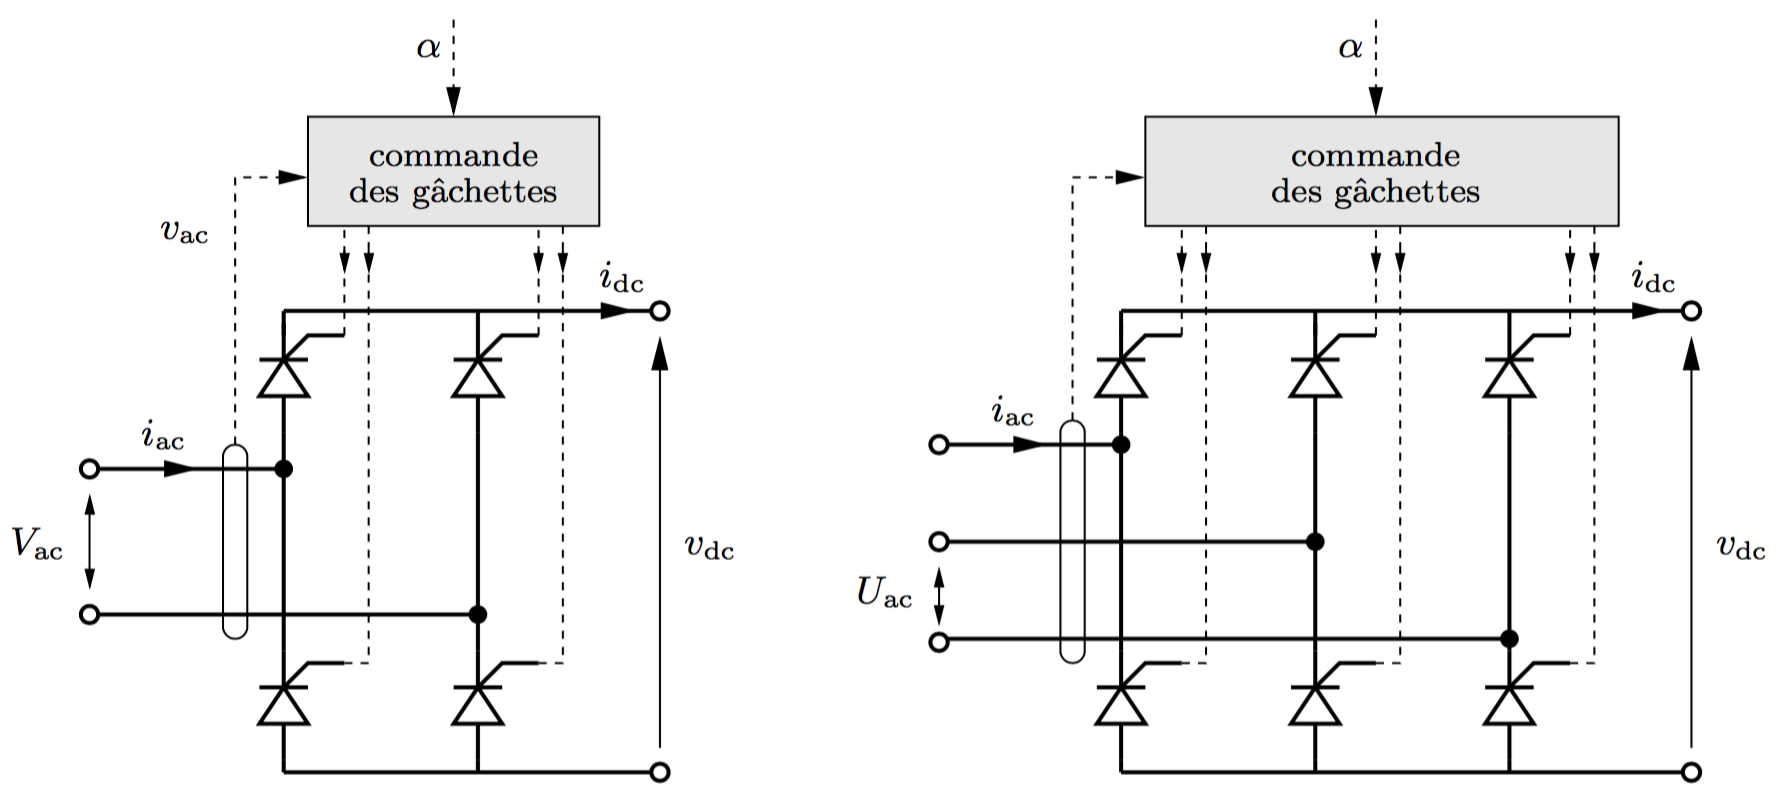
\includegraphics[scale=0.3]{ch3/5}
		\captionof{figure}{} 
		\end{wrapfigure}
		The layouts of these bridges are in the figure. The drive of the thyristors will control a parameter $\alpha$. This $\alpha$ is the lag of the beginning of conduction in the thyristor rectifier with respect to that of a diode rectifier with the same topology ($\alpha = 0$ for a diode). The distortion of the AC and DC quantities are composed of the same order of harmonics. We will consider a load inductive enough to avoid the discontinuity of the current.
		Depending on $\alpha$, we will have a rectifier or an inverter. A DC load able to furnish power will be required for the system to operate as an inverter. 
		
			\subsection{Rectifier operation}
				\subsubsection{Single-phase bridge and RLE load}
					We will assume an ideal AC voltage source. Under these conditions, a rectified current will only appear if $E_{dc} < V_{dc}$. \\
					
					\begin{itemize}
					\item[•] \textbf{Infinitely inductive load}\\
					In \autoref{fig:3.6} we can observe the shapes of the waves for $\alpha \approx 45^{\circ}$. We note that when $v_{ac}$ goes trough 0 to become positive, Th2 and Th3 keep conducting because of the inductance and the thyristors waiting for their initiation. Once booted, conduction begins instantaneously and the other pair of thyristors is inversely-biased. A perfectly smooth $I_{dc}$ implies that $i_{ac}$ is a square-wave current. Nevertheless, the fundamental component $i_{ac,1}(t)$ is shifted with respect to $v_{ac}(t)$  by an angle $\varphi _1 = \alpha$. This induces a reactive power consumption proportional to $\sin \alpha$. Furthermore, we have $I_{ac,1} = \frac{2\sqrt{2}}{\pi}I_{dc}$. We must point out that a discontinuity of $i_{dc}(t)$ when $v_{dc}(t)<0$ is avoided because we used a big inductance (even if $\alpha \neq 0$). 
					\end{itemize}
					
					\begin{center}
					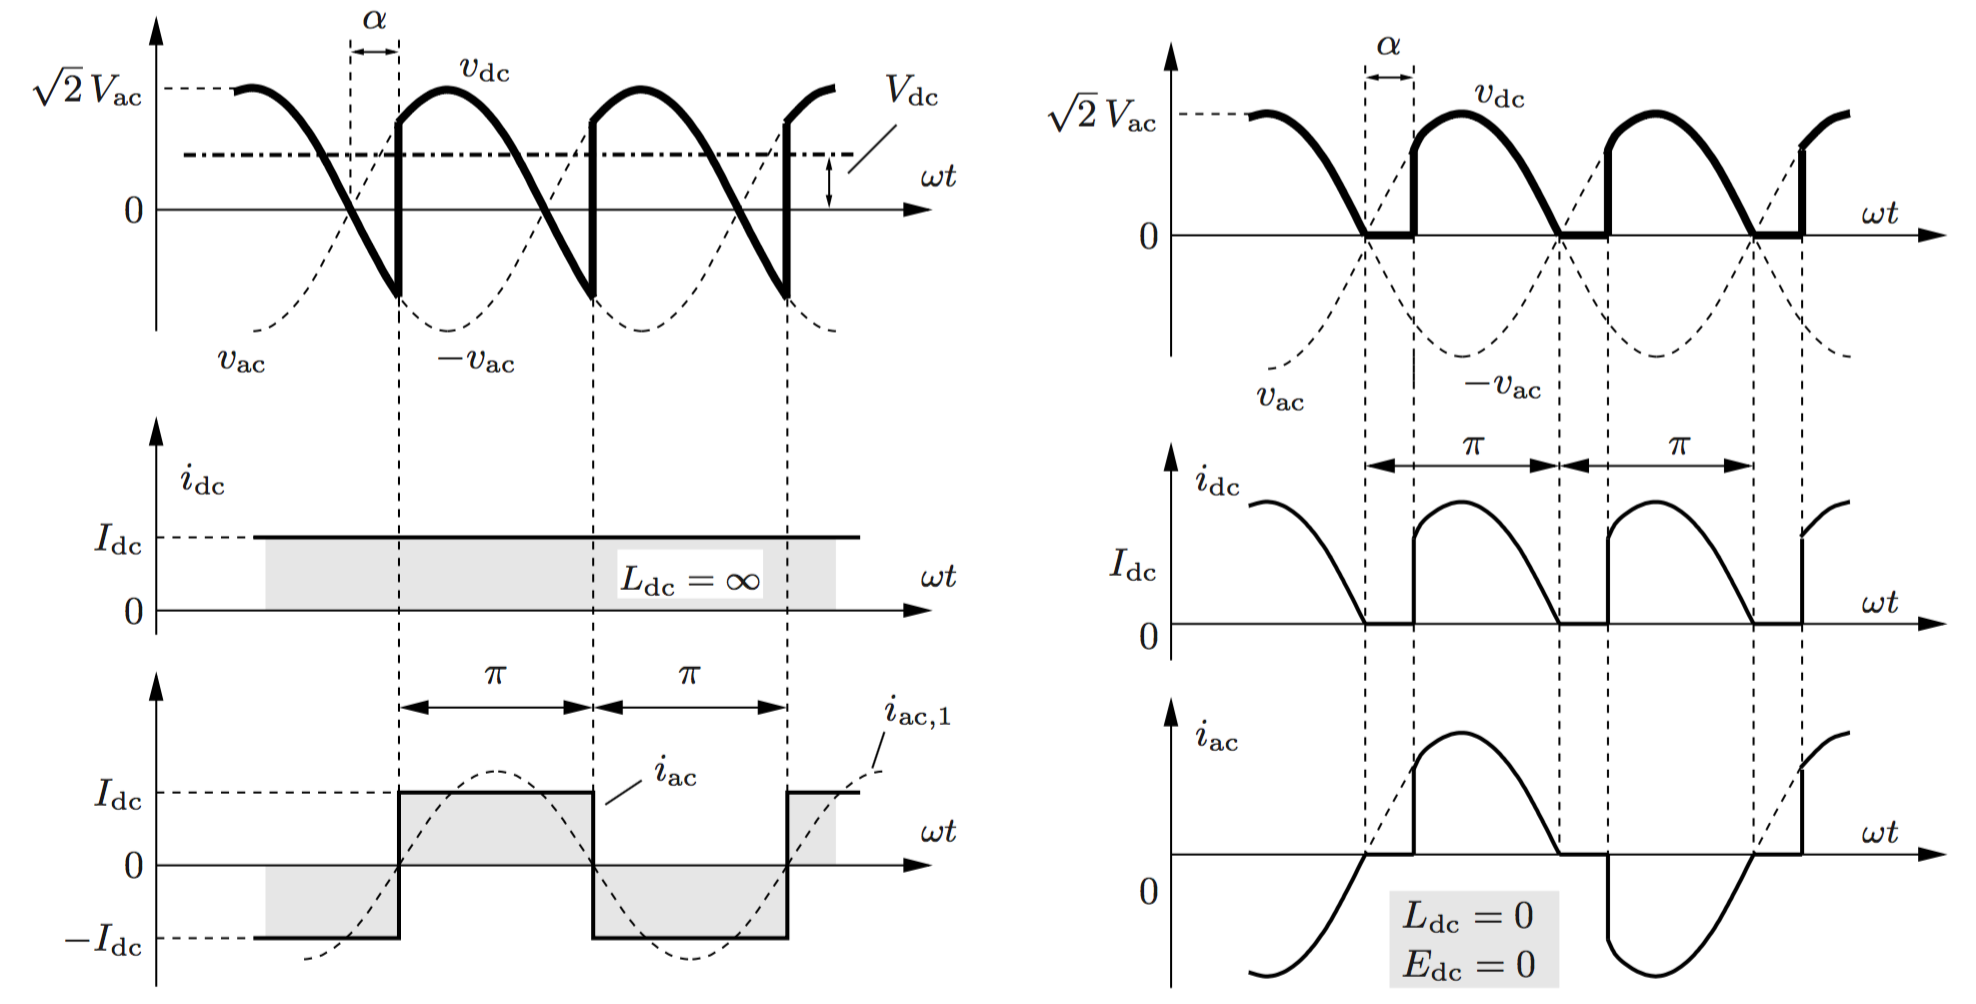
\includegraphics[scale=0.3]{ch3/6}
					\captionof{figure}{}
					\label{fig:3.6}
					\end{center}
					
					\begin{itemize}
					\item[•] \textbf{Purely resistive load}\\
					In this case, conduction becomes discontinuous regardless of the choice of $\alpha$. This happens because neither the current nor the output voltage can invert (see in \autoref{fig:3.6} to the right). 
					\end{itemize}
					
				\subsubsection{Three-phase bridge and infinitely inductive load}
					\begin{wrapfigure}[12]{l}{5.5cm}
					\vspace{-5mm}
					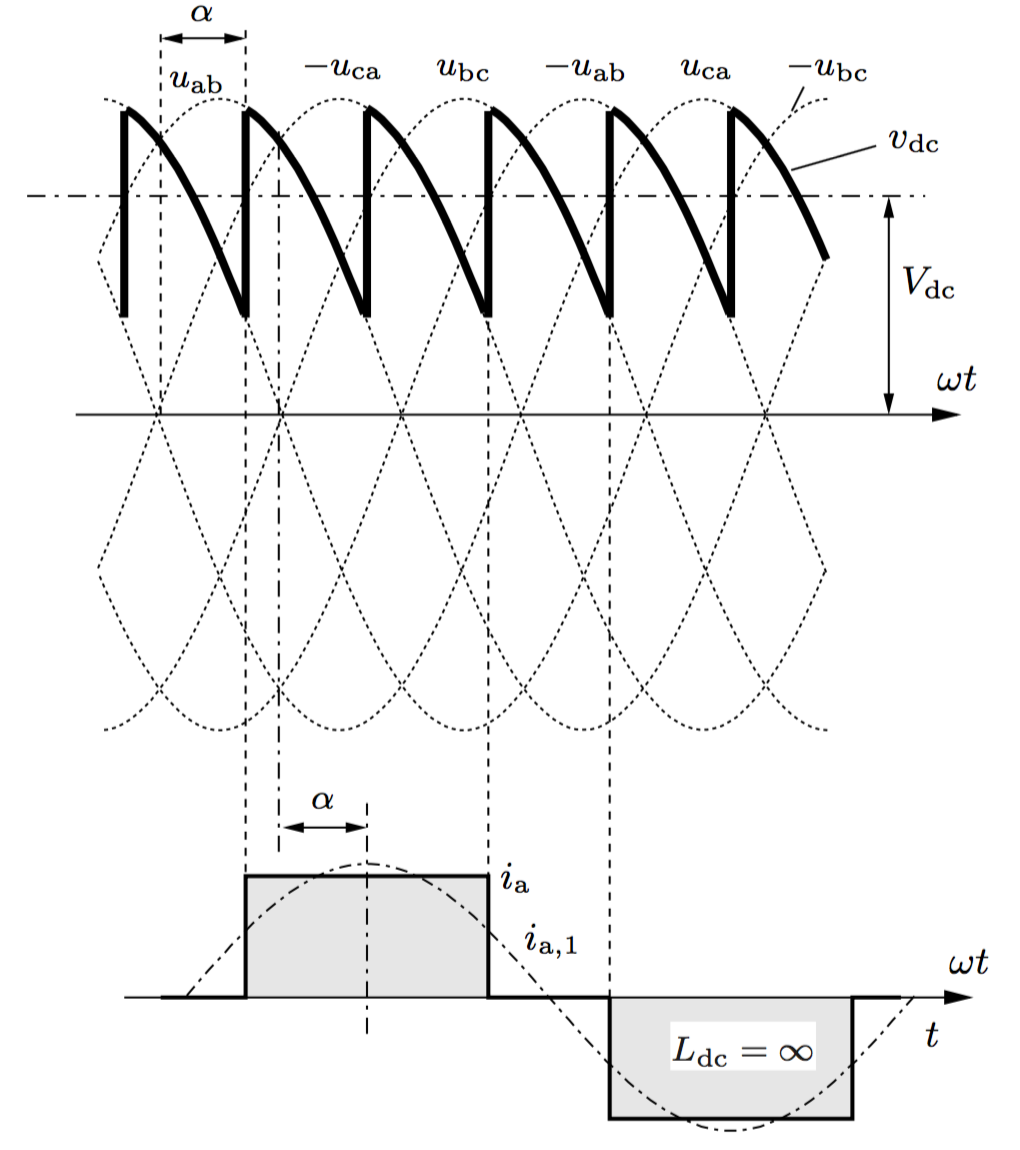
\includegraphics[scale=0.28]{ch3/7}
					\captionof{figure}{} 
					\end{wrapfigure}
					Here, we have the wave shapes when $\alpha \approx 40^\circ$. Under these conditions, the presence of a big inductance will induce a three-phase square wave current $i_{ac}(t)$ with a lag of $\phi _1 = \alpha$ with respect to the phase-to-neutral voltage of the first phase. We have $I_{ac,1} = \frac{\sqrt{6}}{\pi}I_{dc}$. it is easy to observe that the output voltage is never $<0$ as long as $\alpha < 60^\circ$ when we have an inductive load. If we had a purely resistive load, then current would be discontinuous. 
					
				\subsubsection{Average output voltage: basic equations (continuous conduction)}
    				If we have continuous conduction we only need to add $\alpha$ to the integration limits of the equivalent diode bridge:				
					\begin{equation}
					\begin{aligned}
					single-phase &: \frac{1}{\pi} \int _{-\pi /2+\alpha}^{\pi /2 +\alpha} \sqrt{2}V_{ac}\cos\omega t\, d\omega t = \frac{2\sqrt{2}	}{\pi} V_{ac}\cos \alpha \\
					three-phase &: \frac{3}{\pi} \int _{-\pi /6+\alpha}^{\pi /6 +\alpha} \sqrt{2}U_{ac}\cos\omega t\, d\omega t = \frac{3\sqrt{2}	}{\pi} U_{ac}\cos \alpha
					\end{aligned}
					\end{equation}
		
					\begin{wrapfigure}[7]{r}{4.7cm}
					\vspace{-5mm}
					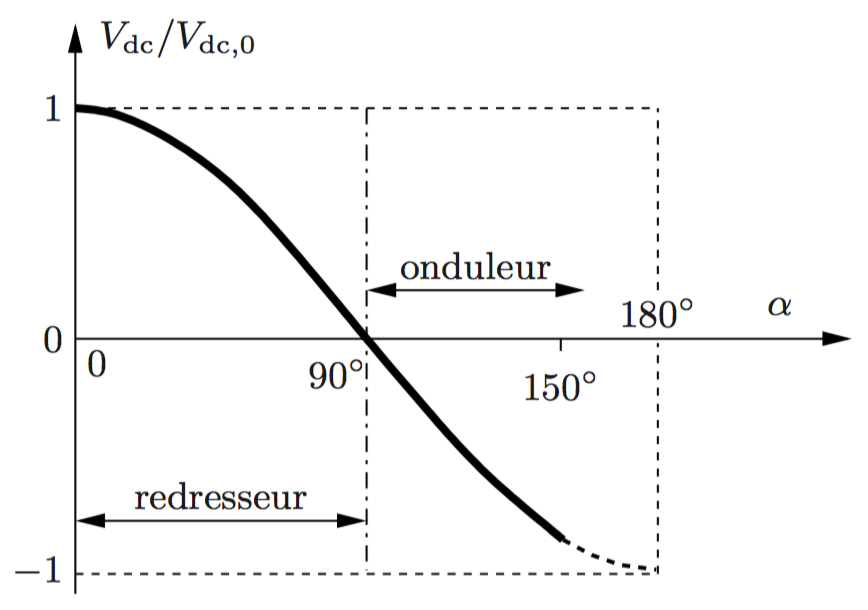
\includegraphics[scale=0.3]{ch3/8}
					\captionof{figure}{} 
					\end{wrapfigure}
					The maximum average corresponds to an $\alpha = 0$ and it will be zero when $\alpha = \pi /2$. If $\alpha > \pi /2$ the average becomes negative. the progression of the average output voltage with $\alpha$ appears in the figure.
					If our source has an inner inductance and if we take into account the conduction losses in the thyristors, the model of the system will become a bit more complex. To simplify it a bit we will use the Thevenin theorem
					
					\newpage
					
			\subsection{Inverter operation (non-autonomous)}
				\begin{wrapfigure}[13]{l}{5.5cm}
				\vspace{-5mm}
				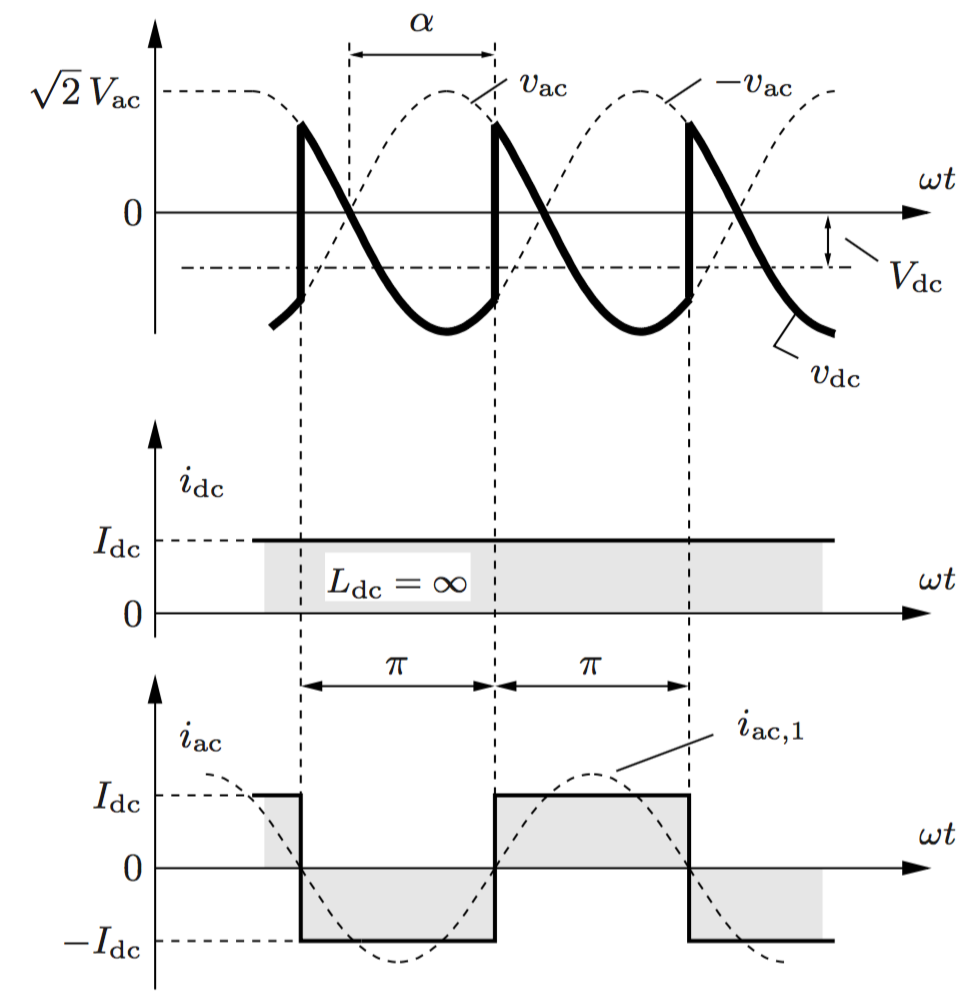
\includegraphics[scale=0.28]{ch3/9}
				\captionof{figure}{} 
				\end{wrapfigure}
				The system operates as an inverter when $\alpha$ is between $90^\circ$ and $180^\circ$. The average output voltage is negative and the average power goes from the DC mesh to the AC mesh. On the side we can see the waves shapes when $\alpha \approx 135^\circ$. Remember: the load must include an energy source such as the \textit{armature of a brushed DC machine}, here we consider a negative $E_{dc}$. As the rectified current is positive, the inequality $E_{dc}<V_{dc}$ is respected:
				\begin{equation}
					V_{dc} = E_{dc} + RI_{dc} \qquad \Rightarrow E_{dc} < V_{dc} < 0 
				\end{equation}
				The theoretical limit of $\alpha$ is $180^\circ$ but it is lower in practice because of the commutation intervals. We note that another AC voltage source is needed in order to control the thyristors. That is why they are called \textbf{semi-controllable} or \textbf{non-autonomous inverters}. Another consequence of the  employment of thyristors is that we are unable to furnish reactive power to the AC grid. 
				
					\subsubsection{Active and reactive power}
						If we consider a very inductive load (or DC source) and we neglect the commutation intervals and the losses in the bridge, the \textbf{active power} of the AC mesh will be:
						\begin{equation}
						\begin{aligned}
						single-phase &: V_{ac}I_{ac,1}\cos \alpha = V_{dc}I_{dc}\\
						three-phase &: \sqrt{3}U_{ac}I_{ac,1}\cos \alpha = V_{dc}I_{dc}.
						\end{aligned}
						\end{equation}

						The \textbf{reactive power} will be: 
						\begin{equation}
						\begin{aligned}
						single-phase &: Q_1 = V_{ac}I_{ac,1}\sin \alpha \geq 0\\
						three-phase &: Q_1 = \sqrt{3}U_{ac}I_{ac,1}\cos \alpha \geq 0.
						\end{aligned}
						\end{equation}
						The rectifier will always draw some reactive power and it will reach a maximum when $\alpha = 90^\circ$. this is the major disadvantage of these converters. The distortion of the output voltage will also be troublesome. For $\alpha = 90^\circ$, $v_{dc}$ will have a sawtooth shape with an average value equal to 0. 
						
	\section{Half controlled bridges (with diodes and thyristors)}
		\begin{wrapfigure}[10]{r}{9cm}
		\vspace{-5mm}
		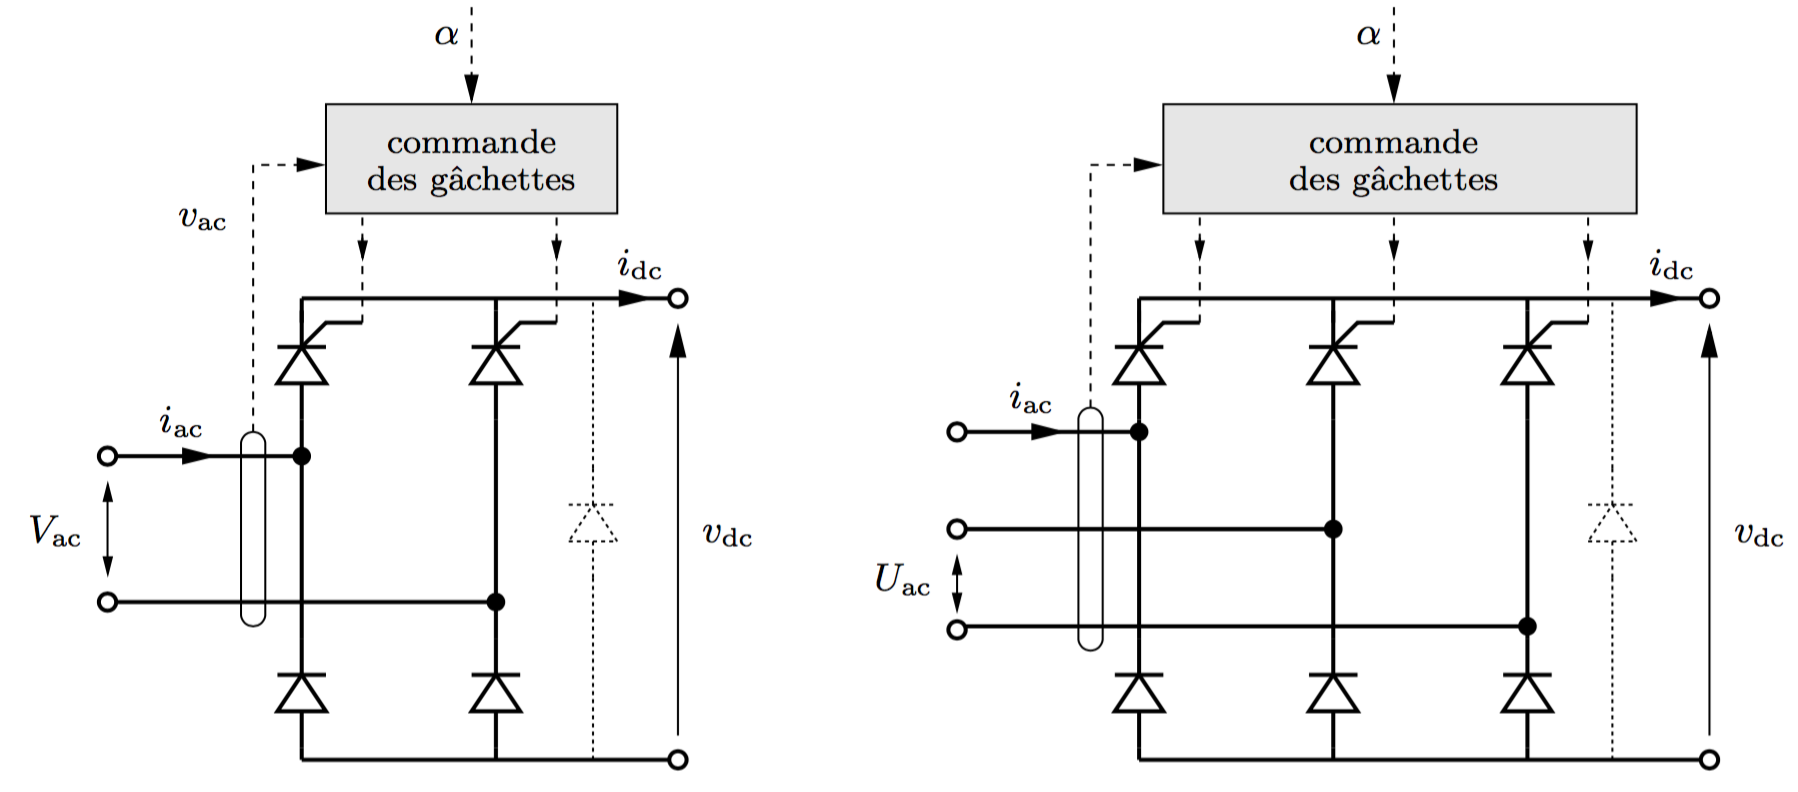
\includegraphics[scale=0.28]{ch3/10}
		\captionof{figure}{} 
		\end{wrapfigure}
		These bridges are composed of diodes and thyristors. We might also add a free-wheeling diode that will not have a big impact on the rectifier. Other than thyristors and diodes other components may be needed depending on the constraints. 
		
		\ \\ First, we will study the case of a single phase bridge with an infinitely inductive load, an ideal AC voltage source and ideal semi-conducting components. The wave shapes are represented in \autoref{fig:3.11}. In that figure we note that $v_{dc}(t)$ cannot be negative. If $\alpha \neq 0$, 
		
		\ \\
		
		\begin{wrapfigure}[12]{l}{5cm}
		\vspace{0mm}
		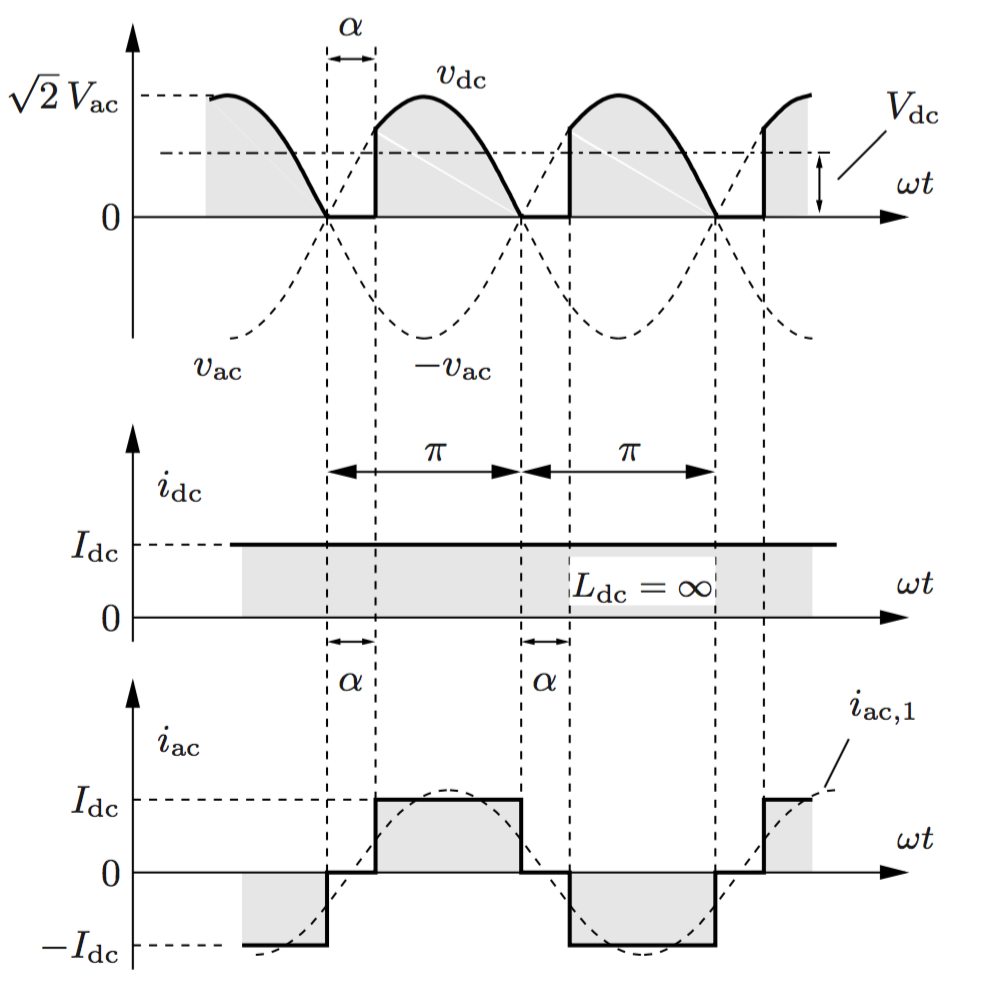
\includegraphics[scale=0.28]{ch3/11}
		\captionof{figure}{} 
		\label{fig:3.11}
		\end{wrapfigure}
		there are intervals without any output voltage. That happens when either the free-wheeling diode or a leg of the bridge short-circuits the system. The average output voltage is given by: 
		\begin{equation}
			V_{dc} = \frac{1}{\pi} \int _{-\pi /2 +\alpha} ^{\pi /2} \sqrt{2} V_{ac} \cos \omega t \, d\omega t = \frac{2\sqrt{2}}{\pi} V_{ac} \frac{1+\cos \alpha}{2}
		\end{equation}
		that means that the average output voltage of a thyristor bridge is the same as the average output voltage of a diode bridge.
		The rms value of the fundamental component of $i_{ac,1}$ is given by: 
		\begin{equation}
			I_{ac,1} = \frac{2\sqrt{2}}{\pi} \cos \frac{\alpha}{2} I_{dc}.
		\end{equation}
		Its lag angle $\phi _1 = \alpha /2$. In addition, the distortion of the AC current will increase $\alpha$. And the power balance will be: 
		\begin{equation}
			V_{ac}I_{ac,1}\cos\alpha /2= V_{dc}I_{dc}. 
		\end{equation}
		In this equation we find the $DPF = \cos \alpha /2$.
		
		As the instantaneous output voltage (and consequently its average) is always positive these bridges cannot work as inverters. Their advantage is a minor cost and complexity. \\
		
		In the case of a three-phase system the average output voltage is: 
		\begin{equation}
			V_{dc} = \frac{3}{\pi} \int _{-\pi /6 + \alpha}^{\pi /6} \sqrt{2} U_{ac} \cos \omega t \, d\omega t = \frac{3\sqrt{2}}{\pi}U_{ac} \frac{1+\cos \alpha}{2}
		\end{equation}
		which is also the average of the output of a diode and a thyristor rectifier.
		
	\section{Characteristics of triacs - AC choppers}
		\begin{wrapfigure}[10]{l}{7cm}
		\vspace{-5mm}
		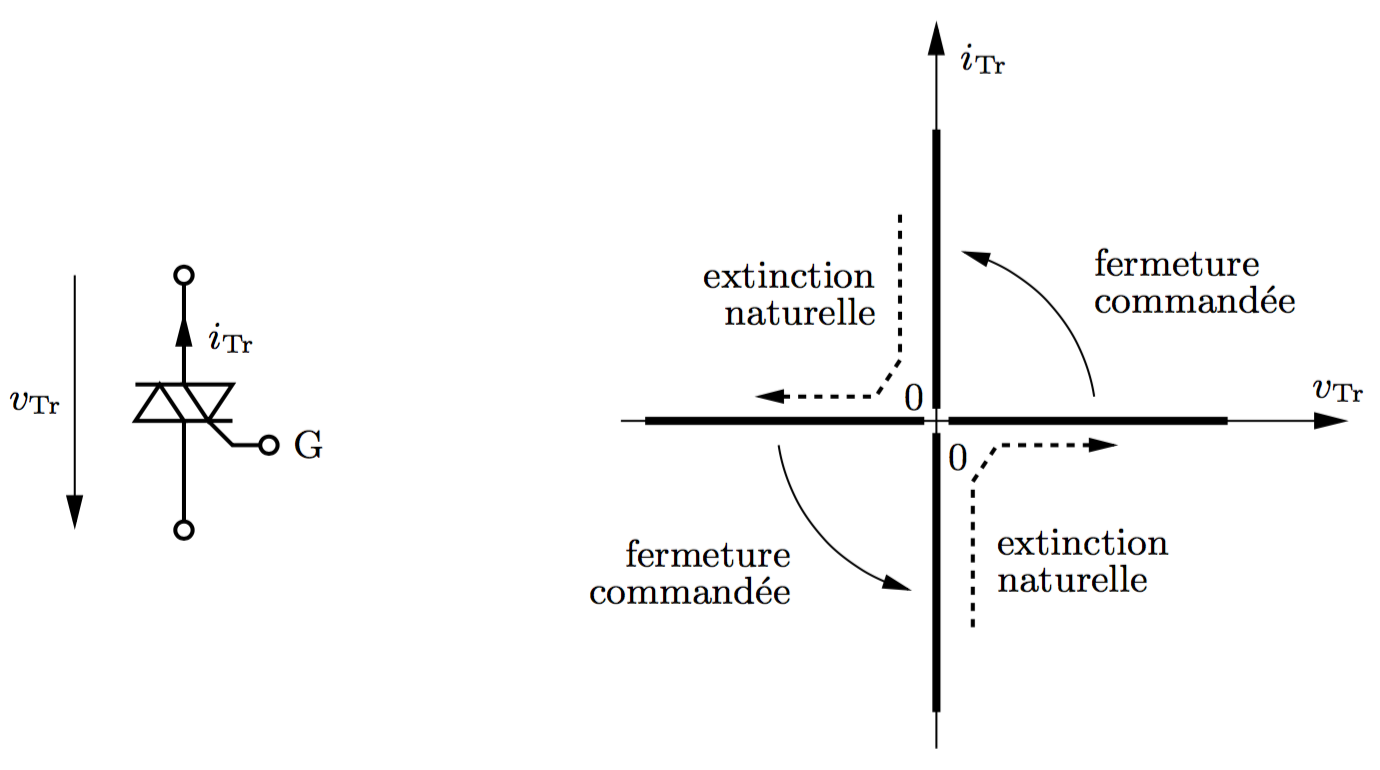
\includegraphics[scale=0.28]{ch3/12}
		\captionof{figure}{} 
		\label{fig:3.12}
		\end{wrapfigure}
		AC choppers carry out AC-AC conversions at a constant frequency whether in single-phase or three-phase. They are composed of triacs or, when the power consumption is too high for triacs, thyristor pairs (anti-parallel connection). This figure shows the bidirectionality of the triacs. In fact, they can conduct in one direction or the other depending on the sign of $v_{Tr}$ when the gate G gets a current impulsion. As triacs are composed of a diode and a thyristor it will turn itself off when the current becomes 0. 
		
			\subsubsection{Single phase AC choppers}
		 	\begin{wrapfigure}[7]{r}{9.8cm}
			\vspace{-5mm}
			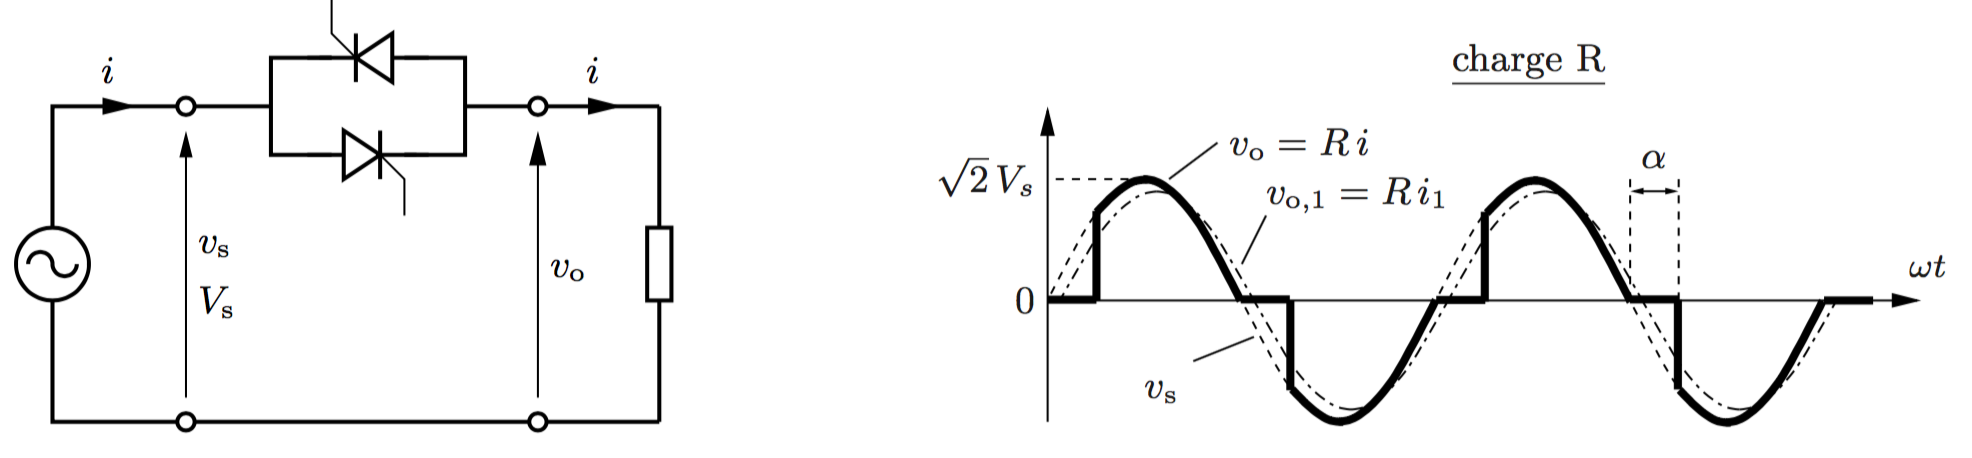
\includegraphics[scale=0.28]{ch3/13}
			\captionof{figure}{} 
			\label{fig:3.13}
			\end{wrapfigure}
			The circuit possesses 2 thyristors set in anti-parallel, which is the same as a triac. The output voltage $v_o(t)$ is controlled by the firing angle $\alpha$. That firing angle represents the time elapsed between the passage through 0 of the input voltage $v_s(t)$ and the sending of an impulsion to the thyristor ($f_o = f_s$). 
			
			\subsubsection{Purely resistive load}
				In \autoref{fig:3.13} we can observe the shapes of $v_o(t)$ and $v_{o,1}(t)$ when we have a purely resistive load $v_o(t) = Ri(t)$. The rms values of the fundamentals will diminish and the shift with respect to $v_s(t)$ will increase with $\alpha$. The chopper will consume reactive power when it feeds solely a load R. The rms value of the fundamental $V_o$ is calculated as follows:
				\begin{equation}
					V_o = \sqrt{\frac{1}{\pi}\int _\alpha ^\pi v_s^2 \, d\omega t} = V_s \sqrt{1- \frac{\alpha}{\pi} + \frac{\sin 2\alpha}{2\pi}}. 
				\end{equation}
				Even harmonics don't appear in the specter because of the half wave symmetry and the THD of $v_o$ will increase with $\alpha$. That is the main disadvantage of choppers. 
	
	\section{Cycloconverters}
		\begin{wrapfigure}[12]{r}{8.3cm}
		\vspace{-5mm}
		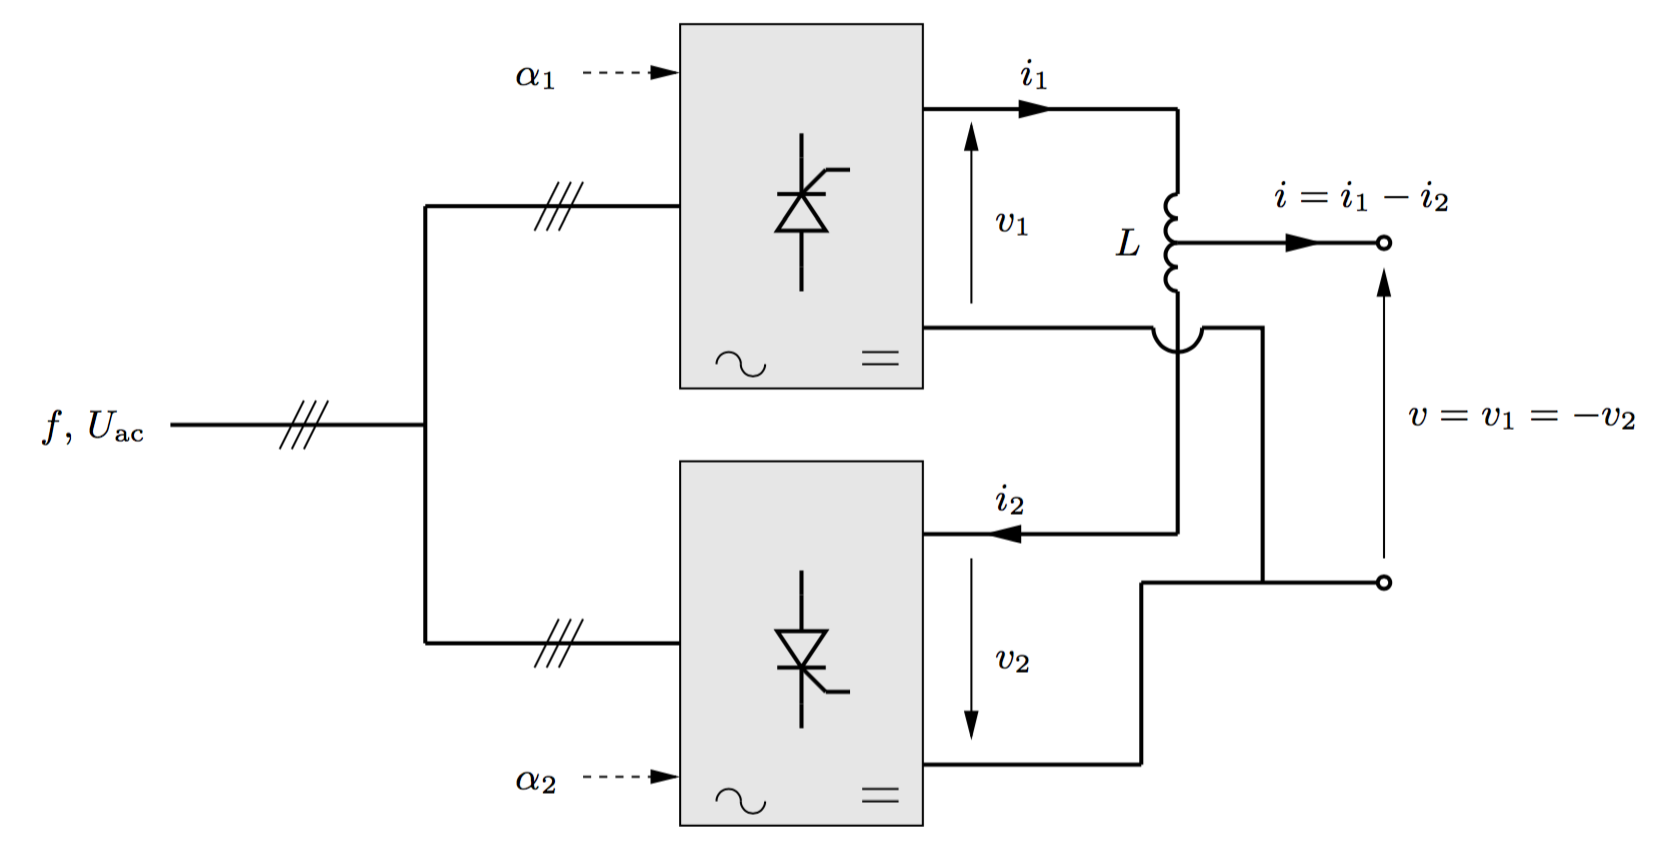
\includegraphics[scale=0.28]{ch3/14}
		\captionof{figure}{} 
		\label{fig:3.14}
		\end{wrapfigure}
		Cycloconverters are \textbf{direct frequency converters}, that is to say it doesn't need a DC bus. They are most often composed of thyristor bridges but it is not the only topology available. Let's consider three-phase to single-phase cycloconverters as the one in the figure. That cycloconverter has two thyristor bridges set head-to-tail. If we change  the firing angle $\alpha_1$ linearly and the firing angle $\alpha_2$ also changes linearly in order to complement $\alpha_1$, that is to say if $\cos \alpha _1 = - \cos \alpha 2$ and $\frac{d|\alpha _1|}{dt} = \frac{d|\alpha _2|}{dt} = \omega _1$, we obtain the average output voltage: 
		\begin{equation}
			v(t) = 1.35 U_{ac} \cos \alpha _1 (t) = 1.35 U_{ac} \cos (\omega _1 t + \gamma). 
		\end{equation}
		As $v_1(t) \neq v_2(t)$, a parasite current appears. The effect of this parasite can be limited through various means such as adding an inductance. We will create our sinusoidal voltage by assembling pieces of the six phase to phase voltages. If the signal isn't too distorted, the fundamental output frequency $f_1$ must be limited to one third or to 40\% of the source frequency. That is shown in this figure. 
		
		\begin{center}
			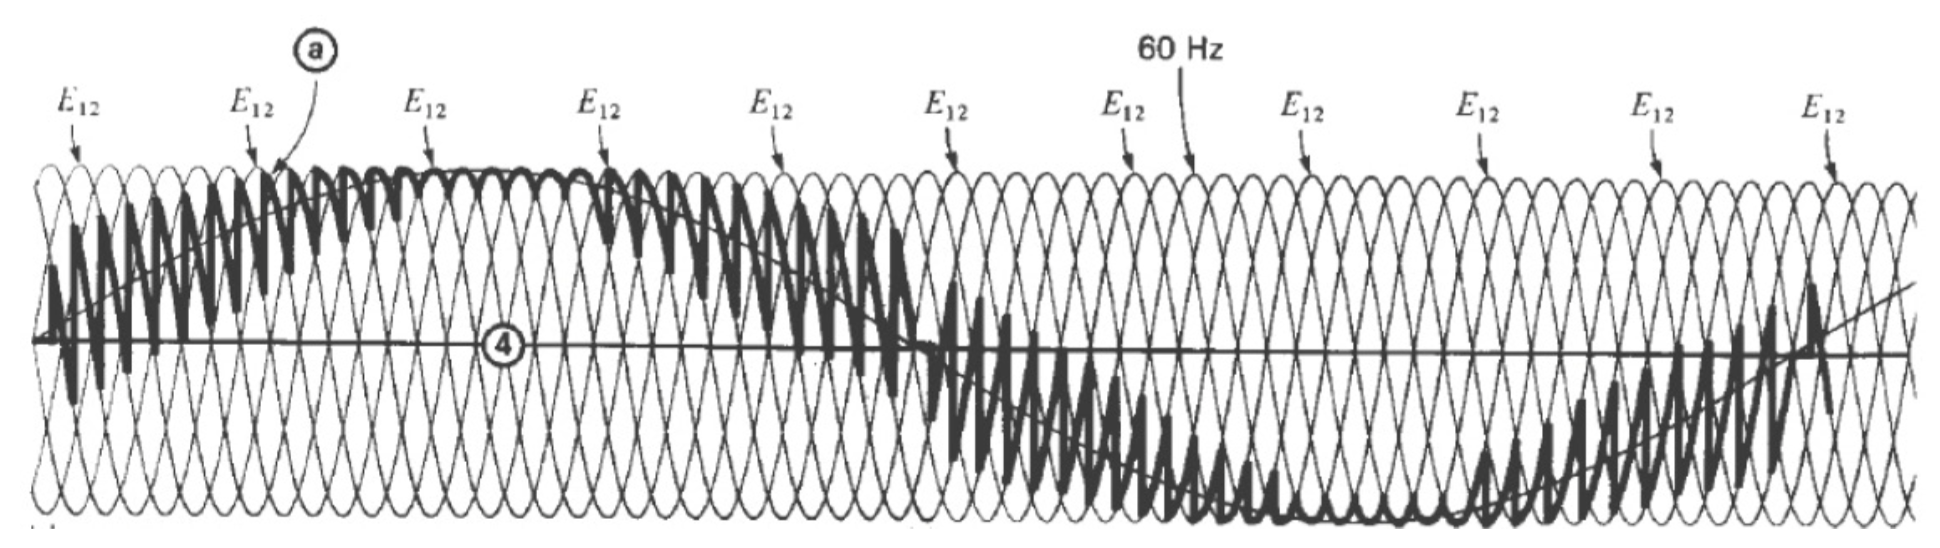
\includegraphics[scale=0.3]{ch3/15}
			\captionof{figure}{}
		\end{center}